\clearpage
\section{Forschungsgrundlage}
\label{sec:research}

Bevor die Forschungsfragen untersucht werden können, muss die theoretische Grundlage gelegt werden.
Zunächst wird analysiert, ob objektorientierte und prozedurale Programmierparadigmen tatsächlich häufiger in Einführungskursen der Informatik verwendet werden als funktionale. Dies soll eine Basis für die Frage schaffen, ob funktionale Programmierung tatsächlich als neuer Ansatz zum Lernen für neue Studierende untersucht werden kann.
Anschließend wird untersucht, wie das Erlernen von Programmierkenntnissen definiert werden kann, und welche Kompetenzen relevant sind. Dies umfasst nicht nur das Schreiben von Code, sondern auch das Lernen der nötigen Denkweisen. Diese theoretischen Konzepte lassen sich in der Theorie des Computational Thinking (CT) zusammenfassen. Demnach müssen auch die Zusammengänge von CT und den Lerntypen betrachtet werden.
Dazu wird CT in diesem Abschnitt exakt für die Arbeit definiert und auf vier häufigste Aspekte reduziert. Zudem wird das Lerntypenmodell, das in dieser Arbeit verwendet wird, erläutert. Dieses dient zur Untersuchung und Kategorisierung der verschiedenen Lernstilausprägungen von Programmieranfangenden.

\subsection{Aktuelle Lerninhalte an Universitäten und Hochschulen}
Umfragen unter Entwickelnden der letzten Jahre haben gezeigt, dass objektorientierte Sprachen noch immer zu den am meisten verwendeten zählen, sowohl im Berufsleben als auch unter Lernenden \cite{stackoverflow}. Dieser Abschnitt untersucht, ob auch an deutschen Universitäten noch vermehrt objektorientierte Paradigmen gelehrt werden.
Darauf aufbauend lässt sich bewerten, ob funktionale Programmierung überhaupt als Alternative in Erwägung gezogen werden kann.

\subsubsection{Übersicht bekannter Paradigmen}
Um die häufig behandelten Paradigmen untersuchen zu können, müssen zunächst die wichtigsten Kategorien definiert werden. Dazu werden die vier verbreitetsten Paradigmen betrachtet \cite{normak}.

\begin{description}
    \item[Imperative Programmierung] Abfolge von Kommandos, die den Zustand des Programms inkrementell ändern. Beschreibungen von Aktionen in einer geregelten Abfolge, ähnlich wie bei einer Anleitung oder einem Rezept.
    \item[Funktionale Programmierung] Orientierung an Funktionen aus mathematischer Sicht. Produzierte Werte sind unveränderlich, und das Programm hat keinen Zustand. Alle Operationen im Programm werden ausschließlich von Funktionen gehandhabt. Die Funktionen sind Objekte erster Klasse und werden wie Daten behandelt.
    \item[Logische Programmierung] Arbeitet mit Axiomen, Schlussregeln und Abfragen auf Basis gegebener Fakten.
    % Axiome - Grundlegende Wahrheiten/Annahmen, die nicht bewiesen werden müssen. Schlussregeln - formale Regeln, nach denen aus gegebenen Axiomen/Fakten neue Wahrheiten abgeleitet werden (z.B Menschen sind sterblich. Sokrates ist ein Mensch. --> Sokrates ist sterblich)
    \item[Objektorientierte Programmierung] Modellierung von echten Objekten im Code. Daten und Funktionen sind in Objekten gekapselt, die durch Klassen organisiert werden. Klassen sind hierarchisch organisiert, etwa durch Vererbung.
\end{description}

\subsubsection{Untersuchung Curricula}\label{sec:curriculares}
Um zu untersuchen, wie verbreitet funktionale Programmierung momentan in Hochschulcurricula ist, wurden 121 Informatik-Studiengänge an verschiedenen Universitäten und Hochschulen in Deutschland untersucht\footnote{Eine detaillierte Beschreibung des Vorgehens befindet sich im Anhang der Arbeit unter \nameref{sec:analysis_curric}.}.
Die Analyse zeigt, dass die Mehrheit der Einführungskurse in der Informatik objektorientierte Programmierparadigmen behandelt\footnote{Der Unterschied der Datensätze "Unspezifisch" und "Keine Infos" wird im Abschnitt \nameref{sec:unspecified_vs_na} näher erläutert.}.

\begin{figure}[H]
    \centering
    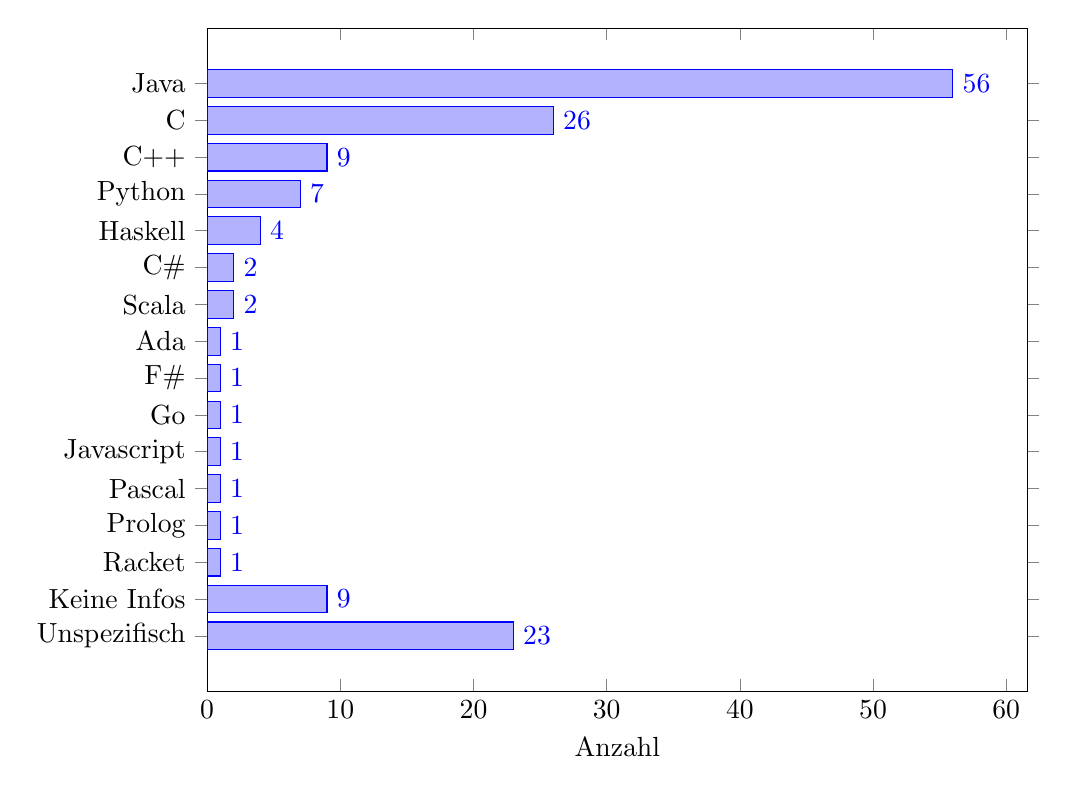
\begin{tikzpicture}
    \begin{axis}[
        xbar,
        width=12cm,
        height=10cm,
        symbolic y coords={{Unspezifisch}, {Keine Infos}, {Racket}, {Prolog}, {Pascal}, {Javascript}, {Go}, {F\#}, {Ada}, {Scala}, {C\#}, {Haskell}, {Python}, {C++},  {C}, {Java}},
        ytick=data,
        nodes near coords,
        xmin=0,
        xlabel={Anzahl}
    ]
        \addplot coordinates {
            (23,{Unspezifisch}) (9,{Keine Infos}) (1,{Racket}) (1,{Prolog}) (1,{Pascal}) (1,{Javascript}) (1,{Go}) (1,{F\#}) (1,{Ada}) (2,{Scala}) (2,{C\#}) (4,{Haskell}) (7,{Python})  (9,{C++}) (26,{C}) (56,{Java})
        };
    \end{axis}
\end{tikzpicture}

    \caption{Zahl der Programmiersprachen in Einführungskursen der Informatik}
\end{figure}

\begin{figure}[H]
    \centering
    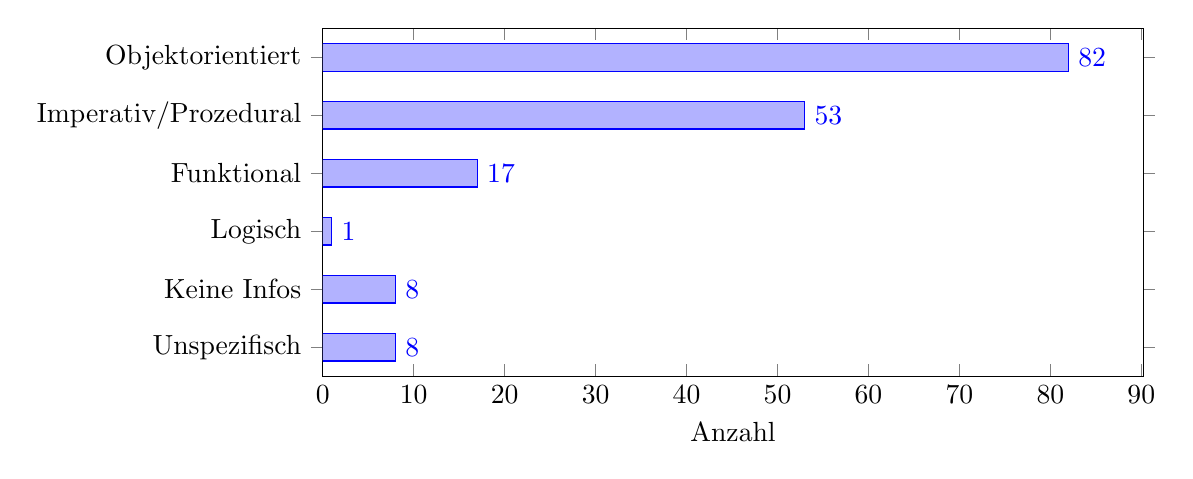
\begin{tikzpicture}
    \begin{axis}[
        xbar,
        width=12cm,
        height=6cm,
        symbolic y coords={{Unspezifisch}, {Keine Infos}, {Logisch}, {Funktional}, {Imperativ/Prozedural}, {Objektorientiert}},
        ytick=data,
        nodes near coords,
        xmin=0,
        xlabel={Anzahl}
    ]
        \addplot coordinates {
            (8,{Unspezifisch}) (8,{Keine Infos}) (1,{Logisch}) (17,{Funktional}) (53,{Imperativ/Prozedural}) (82,{Objektorientiert})
        };
    \end{axis}
\end{tikzpicture}
    \caption{Zahl der Paradigmen in Einführungskursen der Informatik}
\end{figure}

In den meisten Fällen wird an Institutionen Java als Einführung in die Programmierung verwendet, und damit größtenteils imperative und objektorientierte Ansätze.
Ein funktionaler Ansatz für Programmiereinsteigende ist in Deutschland bislang kaum etabliert.

\subsection{Computational Thinking}
Um zu definieren, welche Aspekte genau zum Erlernen von Programmierkenntnissen nötig sind, müssen die einzelnen Aspekte von CT betrachtet und definiert werden. Anschließend können auf Basis der Recherche Vor- und Nachteile in der Anwendung und Erlernung von CT der einzelnen Lerntypen untersucht werden.

\subsubsection{Definition}
Der Begriff CT wurde erstmals 1980 verwendet \cite{papert}, schlussendlich allerdings erst 2006 wieder weitläufig durch eine Kolumne in den öffentlichen Diskurs gebracht \cite{wing2006}.
Grund der erneuten Popularisierung des Begriffes war unter anderem die Diskussion von CT im Kontext von Schulcurricula und die Wichtigkeit des Konzeptes im Alltag.
Da es keine einheitliche Definition von CT gibt, wurden im Kontext der Arbeit verschiedenste Studien betrachtet und verglichen. Es wurde sich zudem an einer Review-Studie aus dem Jahre 2017 orientiert, die bisherige Forschungsergebnisse abwägt und vergleicht \cite{schute}.
\\
In den frühesten Definitionen von CT wird das Konzept häufig als Grundlage für alle unsere Prozesse im Alltag beschrieben. CT ist demnach nicht nur eine Fähigkeit, die nützlich für Entwicklenden ist, sondern begegnet uns überall im Leben \cite{khine17}. Besonders frühere Berichte stellen hervor, dass Informatik nicht nur bedeutet, dass man programmieren kann, sondern dass man Kompetenzen erwirbt, die sich auch in allen anderen Bereichen, sogar künstlerischen Feldern, anwenden lassen \cite{wing2006}.
Auch wird der Begriff im Kontrast zu mathematischem Denken gestellt, und besonders welche Unterschiede und Gemeinsamkeiten die beiden Konzepte haben.

\subsubsection{Computational Thinking Aspekte}
Aufgrund dessen, dass es keine einheitliche Definition von CT gibt, wurden im Rahmen der Arbeit verschiedenste Paper zum Thema analysiert. 2017 wurde eine einheitliche Definition der Aspekte des CT, sowie ein Vergleich aller bisherigen CT-Studien veröffentlicht, an der sich größtenteils in dieser Arbeit orientiert wird \cite{schute}.
Obwohl es viele verschiedene Definitionen von CT gibt, kommen diese letztendlich auf ähnliche Ergebnisse. Vier Aspekte werden demnach immer wieder erwähnt \cite{schute}.

\begin{description}
    \item[Dekomposition] Dieser Aspekt beschreibt die Kompetenz, die Zusammenhänge in einem größeren Problem zu verstehen und dieses in kleinere Teile herunterzubrechen. Durch iteratives Lösen dieser kleineren Teilprobleme kann eine größere Aufgabe oder ein komplexes System angegangen werden.
    \item[Abstraktion] Im ursprünglichen Paper von Wing \cite{wing2006} wird Abstraktion als eine Kernbasis für CT genannt. Hierbei fließt ein weiterer Aspekt ein, die Verallgemeinerung.
    Demnach muss man in der Lage sein, ein komplexes Problem oder System abstrahieren zu können und auf wesentliche Aspekte zu reduzieren. Wing unterscheidet zwischen Abstraktion in jeweiligen Ebenen, Abstraktion als Ganzes und Verbindung zwischen den Ebenen \cite{wing2008}. Ein weiterer häufig erwähnter Aspekt ist die Mustererkennung, die in dieser Arbeit als Unterkategorie der Abstraktion zugeordnet wird.
    \item[Algorithmen] Je nach Forschenden wird dieser Aspekt auch als algorithmisches Denken bezeichnet und soll sich so unter anderem von anderen Denkweisen, wie beispielsweise dem mathematischen Denken, abheben \cite{schute}. Der Aspekt beschreibt die schrittweise Entwicklung eines Lösungsweges für ein Problem, sodass dieses allgemein und immer wieder lösbar durch einen Menschen oder einen Computer ist. Weitere Denkweisen, die mit CT verbunden werden können, sind wissenschaftliches sowie logisches Denken \cite{curzon}.
    \item[Debugging] Dieser Aspekt wird auch teilweise als Evaluation \cite{curzon} oder systematisches Testen \cite{wing2006} bezeichnet. Er beschreibt die Analyse der Lösung. Debugging kann zudem dabei helfen, die Lösung zu verallgemeinern, damit diese wieder auf zukünftige Probleme angewandt werden kann.
\end{description}

Es wird zudem argumentiert, dass es noch weitere Aspekte gibt, die für CT allgemein relevant sind \cite{curzon}. Diese Aspekte können teilweise unter den bereits genannten einsortiert werden.

\begin{description}
    \item[Menschliches Denken] Neben algorithmischem, logischem und wissenschaftlichem Denken gibt es laut Curzon und McOwan \cite{curzon} noch den abstrakteren, menschlichen Aspekt. Ein Algorithmus muss sich danach richten, was ein Nutzender verstehen und realistisch im Alltag anwenden kann.
    \item[Heuristik] Neben der Modellierung eines Algorithmus muss laut Curzon und McOwan noch abgewägt werden, ob sich die Lösung auch tatsächlich realistisch umsetzen lassen kann. Falls nötig, muss ein Problem weiter abstrahiert werden, um eine geeignete Lösung zu finden. Diese ist dann möglicherweise nicht perfekt, aber löst das Problem schneller und effizienter als eine Alternative, die gar nicht in einem realistischen Zeitraum entwickelt werden kann.
    \item[Kreativität] Curzon und McOwan argumentieren, dass Kreativität trotz der scheinbar geringen Zusammenhänge zu Computerwissenschaften als wichtiger Aspekt des CT angesehen werden sollte. Demnach ist Kreativität beispielsweise bei dem Entwurf eines Algorithmus relevant, oder auch bei der Abstraktion. Verallgemeinerung und Mustererkennung erfordern laut den Autoren manchmal große Sprünge, um eine Lösung für ein Problem zu finden, das möglichst effizient und zufriedenstellend für die Nutzende in der realen Welt ist. Dies ist besonders wichtig, wenn für ein spezielles Problem eine völlig neue Lösung entwickelt werden muss.
    \item[Modellierung] Dieser Aspekt kann als Teil von Abstraktion eingeordnet werden. Modellierung eines komplexen Problems oder Systems kann demnach dabei helfen, dieses in einen größeren Kontext einzuordnen und zu verallgemeinern. Hierbei geht es nicht um grafische Modellierung, sondern um die Übertragung realer Probleme in ein virtuelles Modell.
    \item[Verallgemeinerung] Als Unteraspekt der Mustererkennung und Abstraktion ist die Verallgemeinerung besonders relevant in der Wiederverwendung bereits gefundener Lösungen. Hierbei ist es wichtig zu erkennen, wann ein Sachverhalt zu einem bereits existierenden Problem abstrahiert werden kann. Mithilfe der Mustererkennung und Abstraktion kann anschließend entschieden werden, welche Lösungen sich wiederverwenden lassen und welche gegebenenfalls angepasst werden müssen.
    \item[Mustererkennung] Ähnlich wie die Verallgemeinerung hilft dieser Aspekt dabei, Ähnlichkeiten in Problemen zu identifizieren und gegebenenfalls auf bereits existierende Lösungen zurückzugreifen. Allerdings unterscheiden sich die Kompetenzen darin, dass Mustererkennung eher dabei helfen kann, Probleme auf bekannte Darstellungen übertragen zu können. Beispielsweise fällt bei ähnlichen Problemen auf, dass beide durch einen Graphen dargestellt und so gegebenenfalls durch dieselben Algorithmen behandelt werden können. Da für die Mustererkennung auch ein gewisser Grad an Abstraktion nötig ist, wird dieser Aspekt als Unterkategorie davon eingeordnet.
    \item[Darstellung] Dieser Aspekt kann auch als Unteraspekt der Abstraktion und Verallgemeinerung gesehen werden. Er beschreibt die Kompetenz, eine geeignete Darstellungsform für ein Problem oder Daten zu finden, die unter Umständen eine neue Sichtweise auf ein Problem geben kann. Hierbei wird ebenfalls hervorgestellt, wie wichtig eine selbst erstellte grafische Darstellung eines Problems beim gedanklichen "Durchbruch" zu einem effizienteren Algorithmus helfen kann.
\end{description}

\begin{figure}[H]
    \centering
    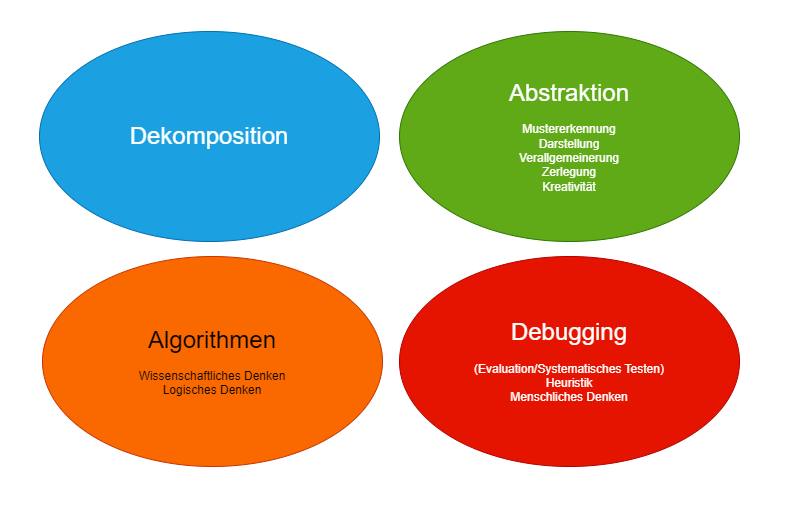
\includegraphics[width=1\linewidth]{Figures/Section_2/CT}
    \caption{Die Haupt- und Unterkategorien Computational Thinking aus verschiedenen Forschungen, grafisch dargestellt}
\end{figure}

Die Arbeit konzentriert sich auf die vier CT Aspekte, die im ersten Abschnitt definiert wurden.

\subsection{Lerntypen}
Um genau zu definieren, welchen Studierenden FP helfen kann, müssen zunächst konkrete Kategorien für die Typen von Lernenden festgelegt werden. Um zu analysieren, welche Studierenden möglicherweise Vorteile beim Erlernen von Programmierung haben könnten, werden diese Kategorien von Lerntypen im Zusammenhang mit CT und den jeweiligen Paradigmen betrachtet.

Ebenso wie im Feld des CT gibt es für Lerntypen kein allgemein akzeptiertes Modell. Allerdings gibt es einige Theorien, die häufiger, besonders im Kontext der Informatik, angewandt werden. Ein verbreitetes Modell ist hierbei das Felder-Silverman Lerntypenmodell (FSLSM) \cite{felder}. 
Das FSLSM wurde speziell im Kontext hoher Abbruchraten in Studiengängen der Ingenieurwissenschaften untersucht, wird allerdings auch vermehrt als Grundlage für Studien im Feld der Informatik verwendet \cite{kumar}.
Um die Lerntypen in der Forschungsgrundlage zu definieren, wird sich an diesem Lerntypenmodell orientiert.

\subsubsection{Differenzierung im Vergleich zu anderen Modellen}
Das FSLSM versteht sich nicht als völlig neues oder umfassendes Modell, und basiert auf bereits existierenden Modellen von etwa Jung \cite{jung}, Kolb \cite{kolb} und Briggs \cite{myers}.
Zudem sind die Lerntypen nicht so eindeutig bestimmbar, wie es herkömmliche Modelle, zum Beispiel das weit verbreitete VARK Modell von N. Fleming suggerieren.
Beispielsweise nutzen alle Menschen sowohl fühlende als auch intuitive Fähigkeiten, bevorzugen allerdings tendenziell eine der beiden Methoden. Das Lernmodell basiert nicht auf festen physischen Merkmalen, sondern auf differenzierteren Präferenzen der Subjekte, und betont, dass schwächere Lerntypendimensionen erlernt werden können.

Das FSLSM beschreibt vier verschiedene Bereiche, in denen sich die Lernstile größtenteils unterscheiden \footnote{Ursprünglich als 5 Bereiche definiert, wobei die Dimension "Inductive Deductive" nachträglich aus dem Modell entfernt wurde. Als Grund hierfür wurde angegeben, dass die meisten Schüler und Studierende einen schlussfolgernden Stil zwar präferieren, aber induktive Methoden in den meisten Fällen laut der Ansicht der Autoren objektiv besser für das Verständnis der Lernenden sind \cite{felder}.}. Hierbei wird immer jeweils ein Gegensatzpaar beschrieben, in das sich Subjekte einsortieren lassen. Die meisten Personen präferieren demnach einen der beiden Stile jeder Kategorie.

% Kurze Zusammenfassung der Lerntypen
\begin{description}
    \item[Sensorisch und Intuitiv] Dieser Aspekt beschäftigt sich damit, wie Personen am besten die Welt um sich herum wahrnehmen können. Hierbei präferieren Personen gewöhnlich eine der beiden Methoden, auch wenn alle Menschen beide verwenden können. Sensorische Typen präferieren, Daten und Fakten auswendig zu lernen, und sich länger mit den Details eines Problems zu beschäftigen. Sie ziehen es vor, einen klar erkennbaren Bezug auf die echte Welt zu haben und Probleme mit etablierten Methoden zu lösen. Intuitive Typen hingegen können ihre Umgebung besser durch eigene Theorien, Vorstellungen und Vermutungen wahrnehmen und setzen auf Innovation und Unsicherheiten. Sie sind besser darin, Abstraktion anzuwenden, und lernen neue Konzepte normalerweise schneller als sensorisch veranlagte Personen.
    \item[Visuell und Verbal] Dieser Aspekt beschäftigt sich mit der Art, wie Personen Input verarbeiten und Informationen am besten verstehen können. Visuelle Typen lernen am besten damit, was sie sehen können, etwa Diagramme, Bilder, Filme und Demonstrationen. Verbale Typen ziehen mehr aus Worten, sowohl geschriebenen als auch gesprochenen Erklärungen. Ihnen können besonders Gruppenarbeiten dabei helfen, das Material zu verstehen. Die Mehrheit der Lernenden hat typischerweise eine stärkere Ausprägung des visuellen Lerntypen, was im Konflikt mit den typischen Stilen von Vorlesungen in den Bereichen Informatik und Ingenieurswissenschaften steht. Hierbei wird meist ein frontaler Input gegeben, der im Großteil auf verbalen Vermittlungen basiert.
    \item[Aktiv und Reflexiv]  Dieser Aspekt beschäftigt sich mit der Verarbeitung von Informationen zum Wissen. Aktive Typen sind demnach besser darin, ihr Wissen direkt in der Anwendung zu vertiefen. Sie präferieren Gruppenarbeiten, in denen sie sich aktiv einbringen können, und lernen mit herkömmlichen Vorlesungsstilen nicht so effektiv. Reflexive Typen hingegen benötigen Zeit, um sich eigenständig mit Inhalten auseinanderzusetzen. Sie ziehen es vor, alleine zu arbeiten, und zuerst alle Fakten durchzudenken, bevor sie ein Problem angehen können.
    \item[Sequenziell und Global] Dieser Aspekt beschäftigt sich mit damit, wie Lernende Zusammenhänge verstehen. Sequenzielle Typen können besser in einer festgelegten logischen Reihenfolge arbeiten, etwa chronologisch, mit einem Buch oder mit den Inhalten einer Vorlesung. Globale Typen hingegen lernen oft sprunghaft und nicht linear, und müssen zunächst eine große Menge an Informationen ansammeln, bevor sich für sie das Gesamtbild erschließt. Da viele herkömmliche Vorlesungsformen auf einer schrittweisen Einführung der Konzepte basieren, haben globale Typen beim Erlernen neuer Sachinhalte normalerweise einen Nachteil gegenüber sequenziellen Lerntypen.
\end{description}
